% !TeX spellcheck = en_US
\documentclass[12pt,a4paper]{article}
\usepackage[utf8]{inputenc}
\usepackage[german]{babel}
\usepackage[T1]{fontenc}
\usepackage{amsmath}
\usepackage{amsfonts}
\usepackage{amssymb}
\usepackage{graphicx}
\usepackage[left=2.5cm,right=2.5cm,top=2cm,bottom=2cm]{geometry}
\usepackage{float}

\usepackage{subcaption}
\usepackage{siunitx}
\usepackage{verbatim} 
\usepackage{flafter}
\usepackage{placeins} %\FloatBarrier

\author{Gruppe A2 \\ Julián Häck, Maria Spethmann}
\title{Protokoll Elektrizitätslehre \\ Physikalisches Grundpraktikum 2}


\begin{document}
	\maketitle
	\thispagestyle{empty} % Keine Seitenzahl auf der Titelseite
	\newpage
	\pagestyle{headings} % Seitenzahlen oben, Section und Subsection in Kopfzeile
	\tableofcontents
	\newpage
\section{Einleitung}
In diesem Versuch werden wir uns mit elektrischen Schwingkreisen beschäftigen. Dazu wird eine Wechselspannung an eine Serien- bzw. Parallelschaltung von je einer Spule einem Kondensator und einem Widerstand angelegt. Das Ziel des Versuch ist es die Güte der Schwingkreise zu bestimmen.
\section{Physikalische Grundlagen}
Beim Wechselstrom gilt für Strom und Spannung im Allgemeinen:
\begin{align}
I(t)=I_0\cdot cos(\omega t - \phi) \qquad und \qquad U(t)=U_0\cdot cos(\omega t)
\end{align}
Mit der Amplitude $I_0$ bzw. $U_0$ und der Phasendifferenz $\phi$.
Für viele Anwendungen ist es sinnvoll die Effektivwerte zu definieren:
\begin{align}
U_eff = \frac{U_0}{\sqrt{2}} \qquad \text{und} \qquad I_eff = \frac{I_0}{\sqrt{2}}
\end{align}
Beim Anlegen einer Wechselspannung an eine Spule oder einen Kondensator muss man beachten, dass diese einen Wechselstromwiderstand darstellen.\\
\textbf{Induktiver Widerstand}
Für den Strom durch eine Spule der Induktivität L ergibt sich:
\begin{equation}
I(t)=\frac{U_0}{\omega L}\cdot cos(\omega t- \frac{\pi}{2})
\end{equation}
und damit die sogenannte Induktanz:
\begin{equation}
X_L=\frac{U_eff}{I_eff}=\omega \cdot L
\end{equation}
\textbf{Kapazitiver Widerstand}
Für die sogenannte Kondensanz gilt analog zur Induktanz:
\begin{equation}
X_C=\frac{U_eff}{I_eff}=\frac{1}{\omega \cdot C}
\end{equation}
\section{Serienschwingkreis}
\subsection{Physikalische Grundlagen}
Für die Impedanz eines Serienschwingkreises gilt nach Kirchhoff:
\begin{equation}
Z=\sqrt{R^2+(\omega L-\frac{1}{\omega C})^2}
\end{equation}
Für die Gütebestimmung durch die Resonanzfrequenz $f_0$ gilt die Thomsonsche Gleichung:
\begin{equation}
f_0=\frac{\omega_0}{2\pi}=\frac{1}{2\pi \sqrt{LC}}
\end{equation}
Um die Güte über die Phasendifferenz von Strom und Spannung zu berechnen benötigt man:
\begin{equation}
tan(\phi)=\frac{\omega L-\frac{1}{\omega C}}{R}
\end{equation}
Des weiteren ist die Güte gleich der Inversen der relativen Resonanzbreite:
\begin{equation}
Q_s=\frac{\omega_0}{\Delta \omega}=\frac{1}{R}\cdot \sqrt{\frac{L}{C}}
\end{equation}
Zu guter Letzt kann man die Güte auch über die Spannungserhöhung an der Spule bestimmt werden:
\begin{equation}
\frac{U_L(\omega_0)}{U(\omega_0)}=\frac{\omega_0 L}{R}=\frac{1}{\omega_0 C R}
\end{equation}
\subsection{Oszilloskop}
\subsubsection{Versuchsaufbau und Durchführung}
Bei der Messung mit dem Oszilloskop wird zum einen die Spannung über den Widerstand und zum anderen die Gesamtspannung abgegriffen. Dabei ist darauf zu achten die Erde so zu platzieren, dass sie für beide Messungen benutzt werden kann.
Nun wird auf dem Oszilloskop die beiden Channel gegeneinander aufgetragen, was in einer Lissajous-Figur resultiert. Wird nun die Eingangsfrequenz variiert kann man diese Figur verändern. Im Resonanzfall sind Strom und Spannung in Phase also ist die Figur eine Gerade. Diese Gerade wird nun eingestellt und anschließend werden die Channel wieder gegen die Zeit aufgetragen. Nun wird die Spannung $U_max$ am Widerstand abgelesen und durch weitere Variation der Frequenz die Spannung von $\frac{U_max}{\sqrt{2}}$ eingestellt. Dies wird für je eine Frequenz oberhalb und unterhalb der Resonanzfrequenz gemacht und aus der Differenz dieser beiden Frequenzen ergibt sich die Breite der Stromkurve und damit die Güte des Schwingkreises.
\subsubsection{Auswertung}
\subsection{CASSY-Messung}
\subsubsection{Versuchsaufbau- und Durchführung}

\subsubsection{Auswertung}

\begin{figure}[H]
	\centering
	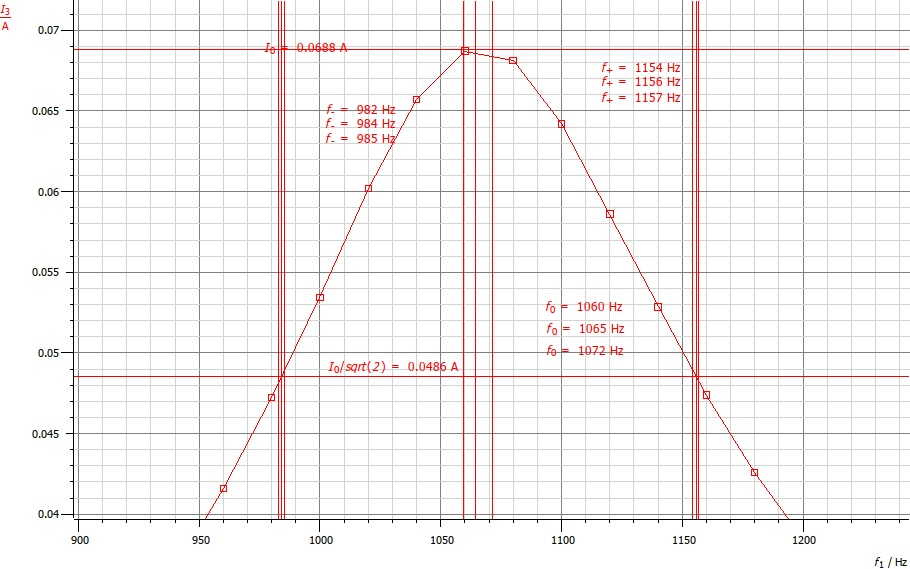
\includegraphics[width=0.8\textwidth]{Daten/S1Ohm_f0.jpg}
	\caption{G"uteberechnung durch Breite des Strommaximums}
	\label{S1Ohm_f0}
\end{figure}
\begin{figure}[H]
	\centering
	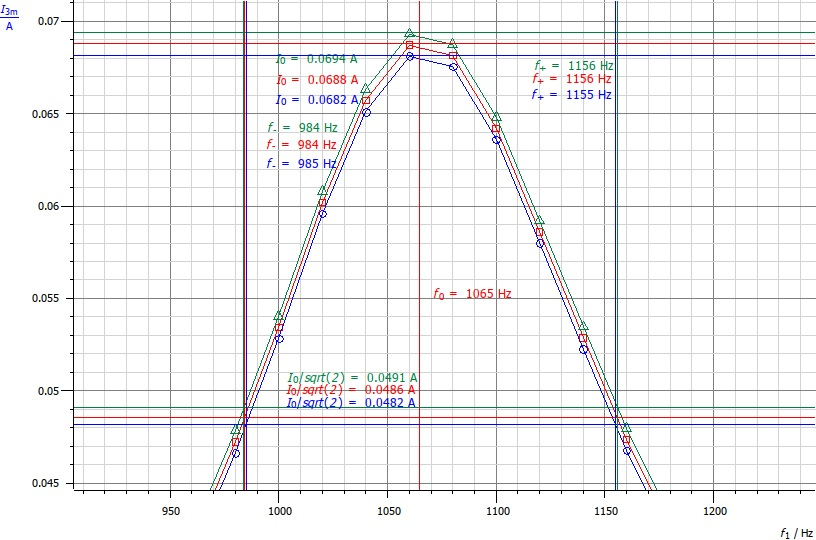
\includegraphics[width=0.8\textwidth]{Daten/S1Ohm_f0_sys.jpg}
	\caption{Verschiebemethode zur Berechnung des systematischen Fehlers}
	\label{S1Ohm_f0_sys}
\end{figure}\begin{figure}[H]
	\centering
	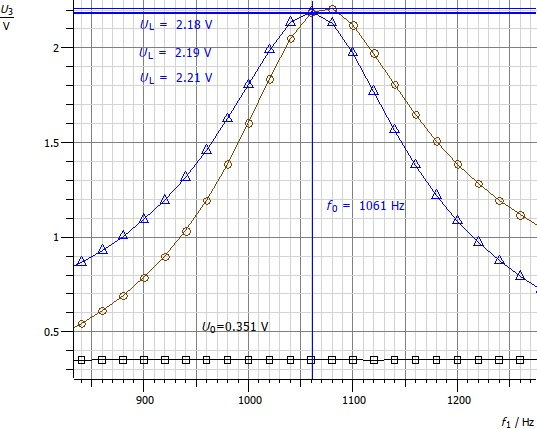
\includegraphics[width=0.8\textwidth]{Daten/S1Ohm_U.jpg}
	\caption{G"uteberechnung durch Ablesen der Spannungsüberhöhung}
	\label{S1Ohm_U}
\end{figure}\begin{figure}[H]
	\centering
	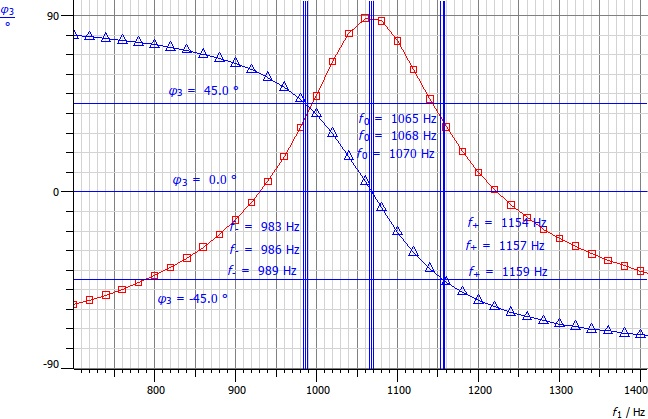
\includegraphics[width=0.8\textwidth]{Daten/S1Ohm_phi.jpg}
	\caption{G"uteberechnung durch Ablesen der Phasenlage}
	\label{S1Ohm_phi}
\end{figure}
\subsection{Zusammenfassung}

\newpage
\section{Parallelschwingkreis}
\subsection{Physikalische Grundlagen}
\subsection{Aufbau und Durchführung}
\subsection{Auswertung}

\begin{figure}[H]
	\centering
	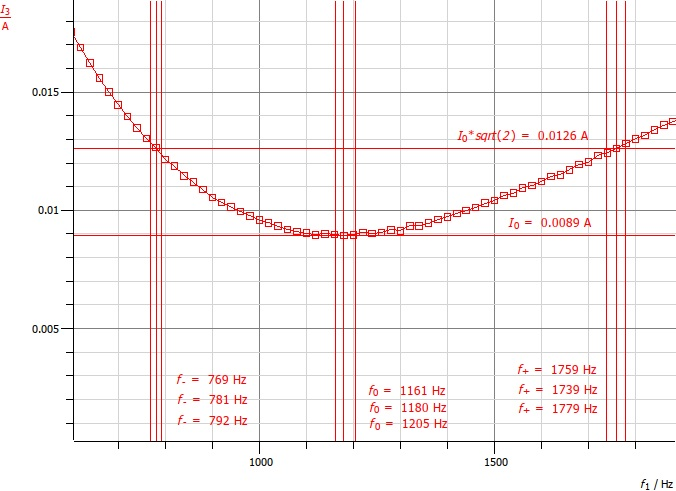
\includegraphics[width=0.8\textwidth]{Daten/P47Ohm_f0.jpg}
	\caption{G"uteberechnung durch Breite des Stromminimums}
	\label{P47Ohm_f0}
\end{figure}

\begin{figure}[H]
	\centering
	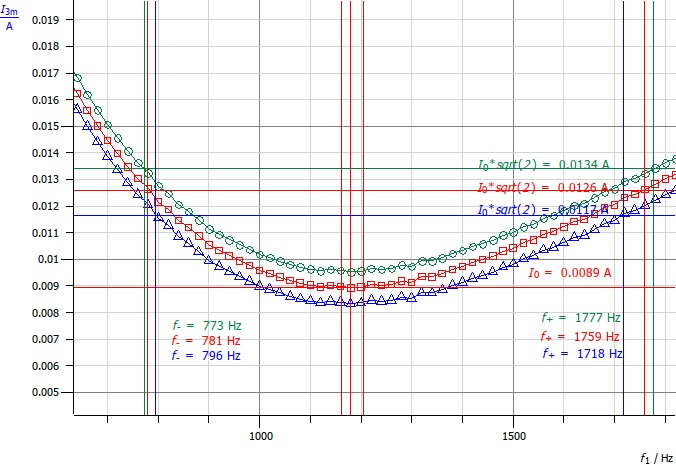
\includegraphics[width=0.8\textwidth]{Daten/P47Ohm_f0_sys.jpg}
	\caption{Verschiebemethode zur Berechnung des systematischen Fehlers}
	\label{P47Ohm_f0_sys}
\end{figure}

\begin{figure}[H]
	\centering
	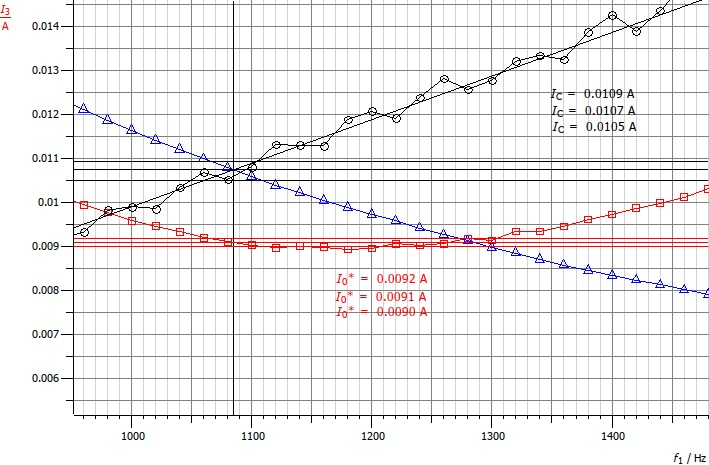
\includegraphics[width=0.8\textwidth]{Daten/P47Ohm_I.jpg}
	\caption{G"uteberechnung durch Ablesen der Stromüberhöhung}
	\label{P47Ohm_I}
\end{figure}
























\subsection{Zusammenfassung}

\end{document}
